\documentclass{ximera}

%\usepackage{todonotes}

\newcommand{\todo}{}

\usepackage{esint} % for \oiint
\ifxake%%https://math.meta.stackexchange.com/questions/9973/how-do-you-render-a-closed-surface-double-integral
\renewcommand{\oiint}{{\large\bigcirc}\kern-1.56em\iint}
\fi


\graphicspath{
  {./}
  {ximeraTutorial/}
  {basicPhilosophy/}
  {functionsOfSeveralVariables/}
  {normalVectors/}
  {lagrangeMultipliers/}
  {vectorFields/}
  {greensTheorem/}
  {shapeOfThingsToCome/}
  {dotProducts/}
  {partialDerivativesAndTheGradientVector/}
  {../productAndQuotientRules/exercises/}
  {../normalVectors/exercisesParametricPlots/}
  {../continuityOfFunctionsOfSeveralVariables/exercises/}
  {../partialDerivativesAndTheGradientVector/exercises/}
  {../directionalDerivativeAndChainRule/exercises/}
  {../commonCoordinates/exercisesCylindricalCoordinates/}
  {../commonCoordinates/exercisesSphericalCoordinates/}
  {../greensTheorem/exercisesCurlAndLineIntegrals/}
  {../greensTheorem/exercisesDivergenceAndLineIntegrals/}
  {../shapeOfThingsToCome/exercisesDivergenceTheorem/}
  {../greensTheorem/}
  {../shapeOfThingsToCome/}
  {../separableDifferentialEquations/exercises/}
}

\newcommand{\mooculus}{\textsf{\textbf{MOOC}\textnormal{\textsf{ULUS}}}}

\usepackage{tkz-euclide}\usepackage{tikz}
\usepackage{tikz-cd}
\usetikzlibrary{arrows}
\tikzset{>=stealth,commutative diagrams/.cd,
  arrow style=tikz,diagrams={>=stealth}} %% cool arrow head
\tikzset{shorten <>/.style={ shorten >=#1, shorten <=#1 } } %% allows shorter vectors

\usetikzlibrary{backgrounds} %% for boxes around graphs
\usetikzlibrary{shapes,positioning}  %% Clouds and stars
\usetikzlibrary{matrix} %% for matrix
\usepackage{pgfplots}
\usepgfplotslibrary{polar} %% for polar plots
\usepgfplotslibrary{fillbetween} %% to shade area between curves in TikZ
\usetkzobj{all}
\usepackage[makeroom]{cancel} %% for strike outs
%\usepackage{mathtools} %% for pretty underbrace % Breaks Ximera
%\usepackage{multicol}
\usepackage{pgffor} %% required for integral for loops



%% http://tex.stackexchange.com/questions/66490/drawing-a-tikz-arc-specifying-the-center
%% Draws beach ball
\tikzset{pics/carc/.style args={#1:#2:#3}{code={\draw[pic actions] (#1:#3) arc(#1:#2:#3);}}}



\usepackage{array}
\setlength{\extrarowheight}{+.1cm}
\newdimen\digitwidth
\settowidth\digitwidth{9}
\def\divrule#1#2{
\noalign{\moveright#1\digitwidth
\vbox{\hrule width#2\digitwidth}}}





\newcommand{\RR}{\mathbb R}
\newcommand{\R}{\mathbb R}
\newcommand{\N}{\mathbb N}
\newcommand{\Z}{\mathbb Z}

\newcommand{\sagemath}{\textsf{SageMath}}


%\renewcommand{\d}{\,d\!}
\renewcommand{\d}{\mathop{}\!d}
\newcommand{\dd}[2][]{\frac{\d #1}{\d #2}}
\newcommand{\pp}[2][]{\frac{\partial #1}{\partial #2}}
\renewcommand{\l}{\ell}
\newcommand{\ddx}{\frac{d}{\d x}}

\newcommand{\zeroOverZero}{\ensuremath{\boldsymbol{\tfrac{0}{0}}}}
\newcommand{\inftyOverInfty}{\ensuremath{\boldsymbol{\tfrac{\infty}{\infty}}}}
\newcommand{\zeroOverInfty}{\ensuremath{\boldsymbol{\tfrac{0}{\infty}}}}
\newcommand{\zeroTimesInfty}{\ensuremath{\small\boldsymbol{0\cdot \infty}}}
\newcommand{\inftyMinusInfty}{\ensuremath{\small\boldsymbol{\infty - \infty}}}
\newcommand{\oneToInfty}{\ensuremath{\boldsymbol{1^\infty}}}
\newcommand{\zeroToZero}{\ensuremath{\boldsymbol{0^0}}}
\newcommand{\inftyToZero}{\ensuremath{\boldsymbol{\infty^0}}}



\newcommand{\numOverZero}{\ensuremath{\boldsymbol{\tfrac{\#}{0}}}}
\newcommand{\dfn}{\textbf}
%\newcommand{\unit}{\,\mathrm}
\newcommand{\unit}{\mathop{}\!\mathrm}
\newcommand{\eval}[1]{\bigg[ #1 \bigg]}
\newcommand{\seq}[1]{\left( #1 \right)}
\renewcommand{\epsilon}{\varepsilon}
\renewcommand{\phi}{\varphi}


\renewcommand{\iff}{\Leftrightarrow}

\DeclareMathOperator{\arccot}{arccot}
\DeclareMathOperator{\arcsec}{arcsec}
\DeclareMathOperator{\arccsc}{arccsc}
\DeclareMathOperator{\si}{Si}
\DeclareMathOperator{\scal}{scal}
\DeclareMathOperator{\sign}{sign}


%% \newcommand{\tightoverset}[2]{% for arrow vec
%%   \mathop{#2}\limits^{\vbox to -.5ex{\kern-0.75ex\hbox{$#1$}\vss}}}
\newcommand{\arrowvec}[1]{{\overset{\rightharpoonup}{#1}}}
%\renewcommand{\vec}[1]{\arrowvec{\mathbf{#1}}}
\renewcommand{\vec}[1]{{\overset{\boldsymbol{\rightharpoonup}}{\mathbf{#1}}}}
\DeclareMathOperator{\proj}{\mathbf{proj}}
\newcommand{\veci}{{\boldsymbol{\hat{\imath}}}}
\newcommand{\vecj}{{\boldsymbol{\hat{\jmath}}}}
\newcommand{\veck}{{\boldsymbol{\hat{k}}}}
\newcommand{\vecl}{\vec{\boldsymbol{\l}}}
\newcommand{\uvec}[1]{\mathbf{\hat{#1}}}
\newcommand{\utan}{\mathbf{\hat{t}}}
\newcommand{\unormal}{\mathbf{\hat{n}}}
\newcommand{\ubinormal}{\mathbf{\hat{b}}}

\newcommand{\dotp}{\bullet}
\newcommand{\cross}{\boldsymbol\times}
\newcommand{\grad}{\boldsymbol\nabla}
\newcommand{\divergence}{\grad\dotp}
\newcommand{\curl}{\grad\cross}
%\DeclareMathOperator{\divergence}{divergence}
%\DeclareMathOperator{\curl}[1]{\grad\cross #1}
\newcommand{\lto}{\mathop{\longrightarrow\,}\limits}

\renewcommand{\bar}{\overline}

\colorlet{textColor}{black}
\colorlet{background}{white}
\colorlet{penColor}{blue!50!black} % Color of a curve in a plot
\colorlet{penColor2}{red!50!black}% Color of a curve in a plot
\colorlet{penColor3}{red!50!blue} % Color of a curve in a plot
\colorlet{penColor4}{green!50!black} % Color of a curve in a plot
\colorlet{penColor5}{orange!80!black} % Color of a curve in a plot
\colorlet{penColor6}{yellow!70!black} % Color of a curve in a plot
\colorlet{fill1}{penColor!20} % Color of fill in a plot
\colorlet{fill2}{penColor2!20} % Color of fill in a plot
\colorlet{fillp}{fill1} % Color of positive area
\colorlet{filln}{penColor2!20} % Color of negative area
\colorlet{fill3}{penColor3!20} % Fill
\colorlet{fill4}{penColor4!20} % Fill
\colorlet{fill5}{penColor5!20} % Fill
\colorlet{gridColor}{gray!50} % Color of grid in a plot

\newcommand{\surfaceColor}{violet}
\newcommand{\surfaceColorTwo}{redyellow}
\newcommand{\sliceColor}{greenyellow}




\pgfmathdeclarefunction{gauss}{2}{% gives gaussian
  \pgfmathparse{1/(#2*sqrt(2*pi))*exp(-((x-#1)^2)/(2*#2^2))}%
}


%%%%%%%%%%%%%
%% Vectors
%%%%%%%%%%%%%

%% Simple horiz vectors
\renewcommand{\vector}[1]{\left\langle #1\right\rangle}


%% %% Complex Horiz Vectors with angle brackets
%% \makeatletter
%% \renewcommand{\vector}[2][ , ]{\left\langle%
%%   \def\nextitem{\def\nextitem{#1}}%
%%   \@for \el:=#2\do{\nextitem\el}\right\rangle%
%% }
%% \makeatother

%% %% Vertical Vectors
%% \def\vector#1{\begin{bmatrix}\vecListA#1,,\end{bmatrix}}
%% \def\vecListA#1,{\if,#1,\else #1\cr \expandafter \vecListA \fi}

%%%%%%%%%%%%%
%% End of vectors
%%%%%%%%%%%%%

%\newcommand{\fullwidth}{}
%\newcommand{\normalwidth}{}



%% makes a snazzy t-chart for evaluating functions
%\newenvironment{tchart}{\rowcolors{2}{}{background!90!textColor}\array}{\endarray}

%%This is to help with formatting on future title pages.
\newenvironment{sectionOutcomes}{}{}



%% Flowchart stuff
%\tikzstyle{startstop} = [rectangle, rounded corners, minimum width=3cm, minimum height=1cm,text centered, draw=black]
%\tikzstyle{question} = [rectangle, minimum width=3cm, minimum height=1cm, text centered, draw=black]
%\tikzstyle{decision} = [trapezium, trapezium left angle=70, trapezium right angle=110, minimum width=3cm, minimum height=1cm, text centered, draw=black]
%\tikzstyle{question} = [rectangle, rounded corners, minimum width=3cm, minimum height=1cm,text centered, draw=black]
%\tikzstyle{process} = [rectangle, minimum width=3cm, minimum height=1cm, text centered, draw=black]
%\tikzstyle{decision} = [trapezium, trapezium left angle=70, trapezium right angle=110, minimum width=3cm, minimum height=1cm, text centered, draw=black]


\outcome{Describe the goals of optimization problems generally.}
\outcome{Find all local maximums and minimums using the First and Second Derivative tests.}
\outcome{Identify when we can find an absolute maximum or minimum on an open interval.}
\outcome{Contrast optimization on open and closed intervals.}
\outcome{Describe the objective function and constraints in a given optimization problem.}
\outcome{Solve optimization problems by finding the appropriate extreme values.}

\title[Dig-In:]{Basic optimization}

\begin{document}
\begin{abstract}
  Now we put our optimization skills to work.
\end{abstract}
\maketitle

An \dfn{optimization problem} is a problem where you need to maximize
or minimize some quantity given some constraints. This can be
accomplished using the tools of differential calculus that we have
already developed.

Perhaps the most basic optimization problems is generated by the
following question:

\begin{quote}
  Among all rectangles of a fixed perimeter, which has the greatest area?
\end{quote}

Let's not do this problem in the abstract, let's do it with numbers.

\begin{example}
  Of all rectangles of perimeter $12$, which side lengths give the greatest area?
  \begin{explanation}
    If a rectangle has perimeter $12$ and one side is length $x$, then
    the length of the other side is $\answer[given]{6-x}$.
    Hence the area of a rectangle of perimeter $12$ can be given by
    \[
    A(x) = x(\answer[given]{6-x}).
    \]
    However, for the side lengths to be physically relevant, we must
    assume that $x$ is in the interval
    $(\answer[given]{0},\answer[given]{6})$. 
      
    So to maximize the area of the rectangle, we need to find the
    maximum value of $A(x)$ on the appropriate interval.
    \begin{quote}
      \textbf{At this point, you should graph the function if you can.}
    \end{quote}
    We'll continue on without the aid of a graph, and use the derivative. Write
    \[
    A'(x) = \answer[given]{6-2x}
    \]
    Now we find the critical points, solving the equation
    \[
    \answer[given]{6-2x} = 0,
    \]
    we see that the only critical point of $A$ is at $x=\answer[given]{3}$
    
    Since $A'(x) = \answer[given]{6-2x}$ is
    \wordChoice{\choice[correct]{positive}\choice{negative}} on
    $(0,3)$ and
    \wordChoice{\choice{positive}\choice[correct]{negative}} on
    $(3,6)$, $x=3$ is where the maximum value of $A$ happens.  This is
      exactly when the rectangle is a square!
  \end{explanation}
\end{example}

A key step to note, is when we explained why $x=3$ is actually the
maximum. Above we basically used facts about the derivative. Below we
use a similar argument.



\begin{example}
  Of all rectangles of area $100$, which has the smallest
  perimeter?
\begin{explanation}
  First we draw a picture, Here is a rectangle with an area of $100$.
\begin{image}
  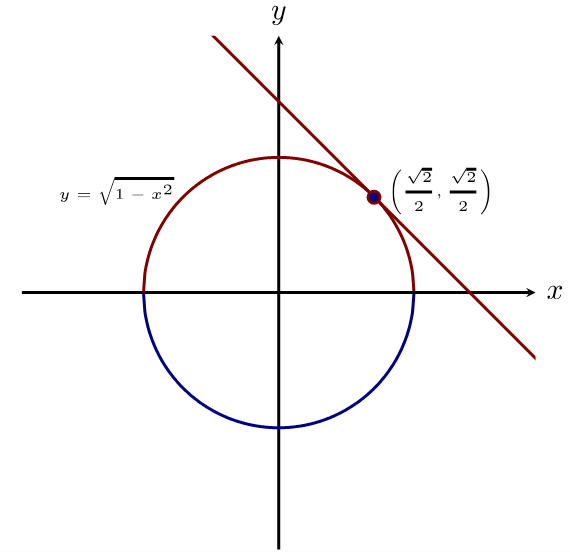
\includegraphics[scale=0.75]{0.png}
\end{image}

If $x$ denotes one of the sides of the rectangle, then the adjacent
side must be $\answer[given]{100/x}$.
 
The perimeter of this rectangle is given by
\[
P(x)=\answer[given]{2x+2\cdot 100/x}.
\]
We wish to minimize $P(x)$.  Note, not all values of $x$ make sense in
this problem: lengths of sides of rectangles must be positive, so
$x>0$. If $x>0$ then so is $100/x$, so we need no second condition on
$x$.
\begin{quote}
  \textbf{At this point, you should graph the function if you can.}
\end{quote}
We next find $P'(x)$ and set it equal to zero. Write
\[
P'(x)=\answer[given]{2-200/x^2} = 0.
\]
Solving for $x$ gives us $x=\pm \answer[given]{10}$. We are interested
only in $x>0$, so only the value $x=\answer[given]{10}$ is of
interest. Since $P'(x)$ is defined everywhere on the interval
$(0,\infty)$, there are no more critical values, and there are no
endpoints. Is there a local maximum, minimum, or neither at $x=10$?
The second derivative is
\[
P''(x)=\answer[given]{400/x^3},
\]
and $P''(10)>0$, so there is a local minimum. Since there is only one
critical point, this is also the global minimum, so the rectangle with
smallest perimeter is the $10\times10$  square.
\end{explanation}
\end{example}


Hence, calculus gives a \textbf{reason} for \textbf{why} a square is
the rectangle with both
\begin{itemize}
\item the largest area for a given perimeter.
\item the smallest perimeter for a given area.
\end{itemize}

We may be done with rectangles, but they aren't done with us. Here is
a problem where there are more constraints on the possible side
lengths of the rectangle.

\begin{example} 
Find the rectangle with largest area that fits inside the graph of the
parabola $y=x^2$ below the line $y=a$, where $a$ is an unspecified
positive constant, with the top side of the rectangle on the horizontal
line $y=a$. See the figure below:
\begin{image}
  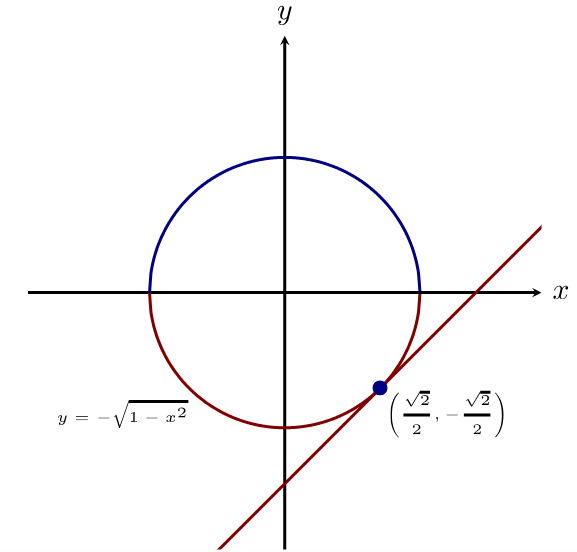
\includegraphics{1.png}
\end{image}
\begin{explanation}
We want to maximize value of $A(x)$.  The lower right corner of the
rectangle is at $(x,x^2)$, and once this is chosen the rectangle is
completely determined. Then the area is
\[
A(x)=\answer[given]{(2x)(a-x^2)}.
\] 
We want the maximum value of $A(x)$ when $x$ is in $[0,\sqrt{a}]$. You
might object to allowing $x=0$ or $x=\sqrt{a}$, since then the
``rectangle'' has either no width or no height, so is not ``really'' a
rectangle. But the problem is somewhat easier if we simply allow such
rectangles, which have zero area as we may then apply the Extreme
Value Theorem and see that we indeed have a maximum and minimum value.
\begin{quote}
  \textbf{At this point, you should graph the function if you can.}
\end{quote}
Setting $0=A'(x)=\answer[given]{-6x^2+2a}$ we find
$x=\answer[given]{\sqrt{a/3}}$ as the only critical point. Testing
this and the two endpoints (as the maximum could also be there), we
have $A(0)=A(\sqrt{a})=\answer[given]{0}$ and
$A(\sqrt{a/3})=\answer[given]{(4/9)\sqrt{3}a^{3/2}}$. Hence, the maximum area
occurs when the rectangle has dimensions $2\sqrt{a/3}\times (2/3)a$.
\end{explanation}
\end{example}

Again, note that above we used the Extreme Value Theorem to guarantee
that we found the maximum.

\end{document}
